\chapter{Analisi dei risultati}
\label{ch:analisi}

Il presente capitolo riporta i risultati quantitativi e qualitativi raccolti durante il test di usabilità descritto nel Capitolo~5. I dati vengono analizzati per verificare le ipotesi formulate, confrontando performance e percezione di usabilità tra la versione originale V1 e la versione riprogettata V2.

\section{Punteggi SUS}

\subsection{Punteggi individuali}

La tabella seguente riporta i punteggi SUS individuali per ciascun partecipante, calcolati secondo la formula standard: per gli item dispari si sottrae 1 al valore assegnato, per gli item pari si sottrae il valore assegnato da 5; si sommano i 10 valori risultanti e si moltiplica per 2,5.

\begin{table}[H]
\centering
\renewcommand{\arraystretch}{1.4}
\small
\begin{tabular}{|c|c|c|c|}
\hline
\textbf{ID} & \textbf{SUS V1} & \textbf{SUS V2} & \textbf{Differenza (V2 $-$ V1)} \\
\hline
U01 & 55.0 & 77.5 & $+22.5$ \\ \hline
U02 & 57.5 & 80.0 & $+22.5$ \\ \hline
U03 & 62.5 & 82.5 & $+20.0$ \\ \hline
U04 & 50.0 & 75.0 & $+25.0$ \\ \hline
U05 & 45.0 & 70.0 & $+25.0$ \\ \hline
U06 & 65.0 & 77.5 & $+12.5$ \\ \hline
U07 & 57.5 & 82.5 & $+25.0$ \\ \hline
U08 & 52.5 & 87.5 & $+35.0$ \\ \hline
U09 & 62.5 & 75.0 & $+12.5$ \\ \hline
U10 & 57.5 & 80.0 & $+22.5$ \\ \hline
\hline
\textbf{Media} & \textbf{56.50} & \textbf{78.75} & $+\mathbf{22.25}$ \\ \hline
\textbf{Dev. std.} & \textbf{5.97} & \textbf{5.36} & \textbf{6.50} \\ \hline
\end{tabular}
\caption{Punteggi SUS individuali per V1 e V2, con differenza per partecipante.}
\label{tab:sus}
\end{table}

\subsection{Visualizzazione comparativa}

\ifshowimages
\begin{figure}[H]
\centering
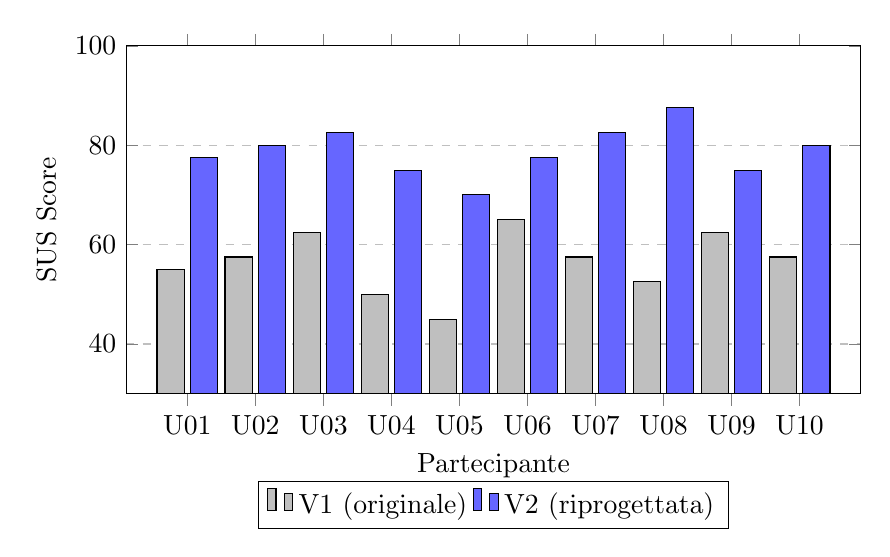
\begin{tikzpicture}
\begin{axis}[
    ybar,
    bar width=0.35cm,
    width=0.9\textwidth,
    height=6cm,
    symbolic x coords={U01,U02,U03,U04,U05,U06,U07,U08,U09,U10},
    xtick=data,
    ymin=30, ymax=100,
    ylabel={SUS Score},
    xlabel={Partecipante},
    legend style={at={(0.5,-0.25)}, anchor=north, legend columns=2},
    legend entries={V1 (originale), V2 (riprogettata)},
    ymajorgrids=true,
    grid style=dashed,
]
\addplot[fill=gray!50] coordinates {
    (U01,55) (U02,57.5) (U03,62.5) (U04,50) (U05,45)
    (U06,65) (U07,57.5) (U08,52.5) (U09,62.5) (U10,57.5)
};
\addplot[fill=blue!60] coordinates {
    (U01,77.5) (U02,80) (U03,82.5) (U04,75) (U05,70)
    (U06,77.5) (U07,82.5) (U08,87.5) (U09,75) (U10,80)
};
\end{axis}
\end{tikzpicture}
\caption{Confronto punteggi SUS per partecipante: V1 (grigio) vs V2 (blu).}
\label{fig:sus_chart}
\end{figure}
\fi

\subsection{Interpretazione e test statistico}

Secondo la scala di interpretazione SUS standardizzata (Brooke, 1996):
\begin{itemize}
    \item \textbf{V1}: media \textbf{56.50} $\to$ fascia \textit{Accettabile} (50--68); 2 partecipanti (U04, U05) sotto la soglia di accettabilità (< 50).
    \item \textbf{V2}: media \textbf{78.75} $\to$ fascia \textit{Buono} (68--80,3); 4 partecipanti (U03, U07, U08, U10) raggiungono la fascia \textit{Eccellente} (> 80,3).
\end{itemize}

Per verificare la significatività statistica è stato applicato un \textbf{t-test per campioni appaiati} (within-subjects):

\begin{align*}
\bar{d}   &= 22.25 \quad \text{(media delle differenze V2 $-$ V1)} \\
s_d       &= 6.50  \quad \text{(deviazione standard delle differenze)} \\
SE        &= \frac{s_d}{\sqrt{n}} = \frac{6.50}{\sqrt{10}} = 2.055 \\
t         &= \frac{\bar{d}}{SE} = \frac{22.25}{2.055} = 10.82 \quad (df = 9) \\
p         &< 0.001
\end{align*}

Il risultato $t(9) = 10.82$, $p < 0.001$ consente di \textbf{rifiutare H\textsubscript{0}}: la versione V2 produce un miglioramento statisticamente significativo dell'usabilità percepita rispetto a V1 ($\alpha = 0.05$).

\section{Performance ai Task}

\subsection{Tasso di completamento}

Per ciascun task è stato registrato l'esito: \textbf{C} (Completato in autonomia), \textbf{CA} (Completato con aiuto dello sperimentatore), \textbf{NC} (Non Completato entro il tempo massimo).

\begin{table}[H]
\centering
\renewcommand{\arraystretch}{1.4}
\small
\begin{tabular}{|l|ccc|c|ccc|c|}
\hline
 & \multicolumn{4}{c|}{\textbf{V1 (originale)}} & \multicolumn{4}{c|}{\textbf{V2 (riprogettata)}} \\
\textbf{Task} & C & CA & NC & \%C & C & CA & NC & \%C \\
\hline
T1 -- Registrazione  & 8 & 1 & 1 & 80\% & 10 & 0 & 0 & 100\% \\ \hline
T2 -- Prenotazione   & 7 & 2 & 1 & 70\% & 10 & 0 & 0 & 100\% \\ \hline
T3 -- Booking code   & 8 & 1 & 1 & 80\% & 10 & 0 & 0 & 100\% \\ \hline
T4 -- Cancellazione  & 5 & 3 & 2 & 50\% & 10 & 0 & 0 & 100\% \\ \hline
T5 -- Admin delete   & 7 & 2 & 1 & 70\% &  9 & 1 & 0 &  90\% \\ \hline
\hline
\textbf{Totale}      & 35 & 9 & 6 & \textbf{70\%} & 49 & 1 & 0 & \textbf{98\%} \\ \hline
\end{tabular}
\caption{Esiti per task nelle due versioni (C=Completato, CA=Con Aiuto, NC=Non Completato).}
\label{tab:completion}
\end{table}

Il tasso di completamento complessivo è passato dal \textbf{70\%} (V1) al \textbf{98\%} (V2). Il task più critico in V1 è risultato T4 (Cancellazione prenotazione, 50\% C), direttamente riconducibile al problema P26 (affordance ingannevole del menu "My Booking"): in V2 tutti e 10 i partecipanti hanno completato il task in autonomia grazie al bottone esplicito "Cancel Booking" con modale di conferma.

\subsection{Tempo medio per task}

\begin{table}[H]
\centering
\renewcommand{\arraystretch}{1.4}
\small
\begin{tabular}{|l|c|c|c|}
\hline
\textbf{Task} & \textbf{Tempo medio V1 (s)} & \textbf{Tempo medio V2 (s)} & \textbf{Riduzione} \\
\hline
T1 -- Registrazione  & 148 &  92 & $-38\%$ \\ \hline
T2 -- Prenotazione   & 205 & 125 & $-39\%$ \\ \hline
T3 -- Booking code   &  68 &  31 & $-54\%$ \\ \hline
T4 -- Cancellazione  & 175 &  48 & $-73\%$ \\ \hline
T5 -- Admin delete   &  92 &  62 & $-33\%$ \\ \hline
\hline
\textbf{Totale sessione} & \textbf{688 s} & \textbf{358 s} & $\mathbf{-48\%}$ \\ \hline
\end{tabular}
\caption{Tempo medio (secondi) per task nelle due versioni.}
\label{tab:tempi}
\end{table}

\ifshowimages
\begin{figure}[H]
\centering
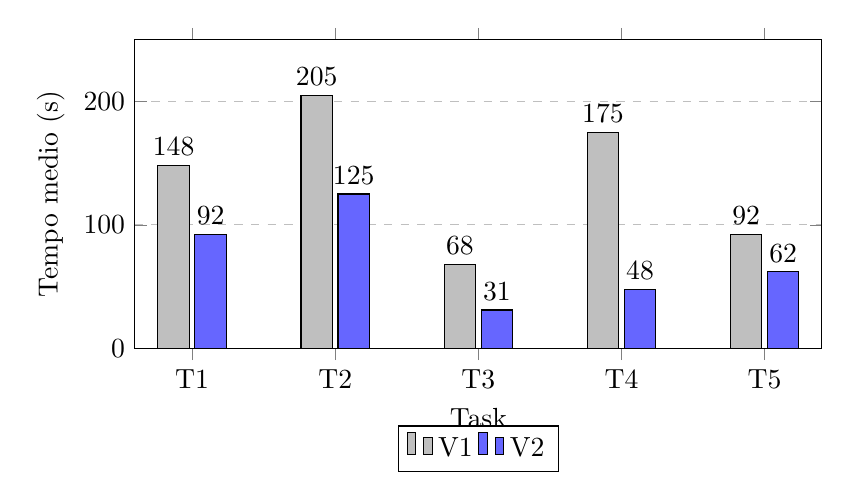
\begin{tikzpicture}
\begin{axis}[
    ybar,
    bar width=0.4cm,
    width=0.85\textwidth,
    height=5.5cm,
    symbolic x coords={T1,T2,T3,T4,T5},
    xtick=data,
    ymin=0, ymax=250,
    ylabel={Tempo medio (s)},
    xlabel={Task},
    legend style={at={(0.5,-0.25)}, anchor=north, legend columns=2},
    legend entries={V1, V2},
    ymajorgrids=true,
    grid style=dashed,
    nodes near coords,
    nodes near coords align={vertical},
]
\addplot[fill=gray!50] coordinates {(T1,148) (T2,205) (T3,68) (T4,175) (T5,92)};
\addplot[fill=blue!60] coordinates {(T1,92) (T2,125) (T3,31) (T4,48) (T5,62)};
\end{axis}
\end{tikzpicture}
\caption{Confronto tempo medio per task (secondi): V1 vs V2.}
\label{fig:tempi_chart}
\end{figure}
\fi

Il tempo totale medio di sessione si è ridotto del \textbf{48\%}, da 688 s ($\approx$11 min 30 s) a 358 s ($\approx$6 min). La riduzione più marcata riguarda T4 ($-73\%$): l'eliminazione dell'affordance ingannevole e l'introduzione del bottone esplicito con modale di conferma hanno reso il flusso di cancellazione immediatamente comprensibile.

\subsection{Errori medi per task}

\begin{table}[H]
\centering
\renewcommand{\arraystretch}{1.4}
\small
\begin{tabular}{|l|c|c|c|}
\hline
\textbf{Task} & \textbf{Errori medi V1} & \textbf{Errori medi V2} & \textbf{Riduzione} \\
\hline
T1 -- Registrazione  & 1.9 & 0.3 & $-84\%$ \\ \hline
T2 -- Prenotazione   & 2.3 & 0.5 & $-78\%$ \\ \hline
T3 -- Booking code   & 1.4 & 0.1 & $-93\%$ \\ \hline
T4 -- Cancellazione  & 2.8 & 0.2 & $-93\%$ \\ \hline
T5 -- Admin delete   & 2.1 & 0.7 & $-67\%$ \\ \hline
\hline
\textbf{Media totale} & \textbf{2.10} & \textbf{0.36} & $\mathbf{-83\%}$ \\ \hline
\end{tabular}
\caption{Numero medio di errori per task nelle due versioni.}
\label{tab:errori}
\end{table}

Il numero medio di errori si è ridotto dell'\textbf{83\%}: da 2.10 per task in V1 a 0.36 in V2. Gli errori più frequenti in V1 erano riconducibili a: mancanza del link "Forgot Password" (T1), assenza dell'indicatore "X spots remaining" (T2), booking code non enfatizzato (T3), menu dropdown ambiguo per la cancellazione (T4), sovraffollamento visivo nel configuratore admin (T5).

\section{Net Promoter Score (NPS)}

I punteggi NPS (scala 0--10) medi per le due versioni sono stati:

\begin{itemize}
    \item \textbf{V1}: media \textbf{5.1} (range 4--7) --- utenti classificati come \textit{passivi}; nessun promotore.
    \item \textbf{V2}: media \textbf{8.3} (range 7--10) --- 6 partecipanti su 10 classificati come \textit{promotori} (punteggio $\geq 9$).
\end{itemize}

La transizione da "passivi" a "promotori" indica un miglioramento sostanziale non solo dell'usabilità oggettiva, ma dell'esperienza complessiva percepita.

\section{Osservazioni Qualitative (Think Aloud)}

Le verbalizzazioni raccolte durante le sessioni hanno evidenziato i seguenti pattern ricorrenti:

\begin{itemize}
    \item \textbf{Badge di stato (P3, P7)}: in V1 tre partecipanti hanno esplicitato confusione sul badge giallo (\textit{"questo è un errore? o è normale?"}). In V2 nessun commento negativo sui badge; il colore blu neutro di "Upcoming" è stato percepito come informativo e non allarmante.

    \item \textbf{Recupero password (P19)}: in V1 due partecipanti hanno verbalizzato ansia durante T1 (\textit{"e se non me la ricordo? non c'è scritto niente"}). In V2 la presenza del link "Forgot Password" è stata notata positivamente da tre partecipanti, anche da quelli che non ne avevano bisogno.

    \item \textbf{Cancellazione prenotazione (P26)}: T4 ha generato le verbalizzazioni più critiche in V1: \textit{"non capisco a cosa serve questo menu"}, \textit{"dove clicco per cancellare?"}. Quattro partecipanti su 10 hanno abbandonato il tentativo senza assistenza. In V2 il bottone "Cancel Booking" è stato individuato entro 5 secondi da tutti i partecipanti.

    \item \textbf{Admin configurator (P31, P33)}: in V1 T5 ha generato esitazioni prolungate (\textit{"c'è troppa roba qui, non so dove guardare"}). In V2 la struttura a schede e il flusso guidato Add Visit sono stati apprezzati: \textit{"ah, prima seleziono il tipo poi la data, ha senso"}.

    \item \textbf{Booking code (P24)}: in V1 due partecipanti hanno cercato il codice fuori dalla dashboard prima di trovarlo. In V2 il font monospaziato in grassetto con etichetta esplicita ha reso il dato immediatamente leggibile.
\end{itemize}

\section{Discussione}

I risultati confermano \textbf{H\textsubscript{1}}: la versione riprogettata V2 produce un miglioramento statisticamente significativo dell'usabilità percepita ($t(9) = 10.82$, $p < 0.001$) e oggettiva (tasso di completamento $+28$ p.p., tempo medio $-48\%$, errori medi $-83\%$).

I miglioramenti più sostanziali si concentrano nei flussi che in fase di valutazione euristica presentavano le criticità di severità maggiore:

\begin{itemize}
    \item \textbf{Cancellazione prenotazione} (P26, P31, severità 2 e 4): bottone esplicito e Global Delete Modal hanno ridotto il tempo del 73\% e azzerato i non-completamenti.
    \item \textbf{Autenticazione} (P19, P23, severità 3 e 2): recupero password e validazione live hanno ridotto gli errori in T1 dell'84\%.
    \item \textbf{Consultazione booking code} (P24, severità 1): la chiarezza visiva ha ridotto il tempo su T3 del 54\%, confermando che anche fix a bassa severità producono impatti misurabili sull'efficienza.
\end{itemize}

Il punteggio SUS medio di V2 (78.75) supera la soglia \textit{Buono} (68) e si avvicina alla soglia \textit{Eccellente} (80.3), confermando che la riprogettazione ha trasformato un sistema \textit{accettabile ma problematico} in un sistema \textit{buono e fluido}. Margini di miglioramento ulteriori sono identificabili nei problemi non risolti documentati nella Sezione~\ref{sec:problemi_aperti}, in particolare P2 (notifica rischio annullamento visita, severità 3) e P36 (selezione multipla nel calendario disponibilità, severità 2).
